\documentclass[12pt]{article}

% Packages
\usepackage{amsmath, amssymb}
\usepackage{graphicx}
\usepackage{geometry}
\usepackage[backend=biber, style=apa]{biblatex} % Use biblatex with biber
\usepackage{wrapfig}
\usepackage{hyperref}
\usepackage{appendix} % For appendix management
\usepackage{booktabs} % For better table lines
%make links look nice


% Page layout
\geometry{a4paper, margin=1in}

% Bibliography file
\addbibresource{references.bib} % Specify the .bib file

% Title and Author
\title{Title of the Paper}
\author{Author Name}
\date{\today}

% ------------------------------------------------------------------------------
% Document
\begin{document}

\maketitle
% 1. Executive Summary
\section*{1. Executive Summary (max half page)}
% Your summary here.

% 2. Introduction
\section*{2. Introduction (about one page)}
\subsection*{(a) Cause and impact of economic fluctuations}
% Content here.

\subsection*{(b) Consequences for economy and why policy should act}
% Content here.

\subsection*{(c) Brief overview of suggested policy}
% Content here.



% ------------------------------------------------------------------------
% THEO ------------------------
% ------------------------------------------------------------------------

% 3. Bird’s Eye View of the Model
\section*{3. Bird’s Eye View of the Model (about two pages)}

\subsection*{(a) Outline of the Model Structure (graphical and verbal, no equations)}
% Content here (include figure environment if needed).
The Dynamic Stochastic General Equilibrium (DSGE) Model used for this policy analysis features
three representative agents, namely a representative household, intermediate goods firm and final goods firm, 
as well as the government. 

The reperesentative household aims to maximize its intertemporal utility, i.e. well-being 
across all periods. It derives utitlity from consumption and its utitltiy is reduced by working. To optimize the its objective
it chooses consumption, labour effort, investment in capital for the in every period. %Ct,Lt,Xt,Mt+1,Bt+1,Kt+1
Furthermore it makes choices that affect the next period,  how much money holdings to save, which determines the money available
in the next period. As well as how many bonds to pay at price $q_t$ which pay off in the next period. (\textbf{Should 
I say here it also chooses} $K_{t+1}$ \textbf{I think that is covered by } $X_t$). When trying to maximize its utility
the reperesentative household faces two constraints. First, to consume it must have cash available beforehand, i.e. only money 
saved in the last period, at 0\% interest compared to $\frac{1}{q} -1$ from the bonds, can be used to buy consumption goods. 
The second constraint is a common budget constraint, which simply requires that income be larger than or equal to expenses. 
The households values utility derived today more highly than that derived in a future period. Thus future utility is discounted. 

The intermediate goods firm as well as the final goods firm maximize their profit. 
The revenue of the intermediate firm stem from selling their intermediate good to the 
final goods firm. The cost incurred consitst of the nominal wage paid to labour, rent paid to capital, both
of which are provided by the household. It is bound by a Cobb-Douglas function with a price stickiness friction, and 
the supply of all intermediate goods must be met by demand for that good from the final good firm. 
As just explained the final good firm buys the intermediate goods. The firm's input are substitutable to some degree. 

The government has fiscal and monetary policy at their disposal, but cannot combine the two. 



\subsection*{(b) Policy Structure of the Model (main equations)}
% Content here (use align or equation environments).

\subsection*{(c) Calibration of the Model}
The model is calibrated to the Canadian economy in 1979, assuming that one period corresponds to a year. 
The discount factor $\beta$ is set to 0.96, inline with \textcite{someOilDemandSupply2023} and close to \textcite{corriganToTEMIIIBank2021}. 
The intertemporal consumption elasticity $\sigma$ is set to less than 1, \textbf{indicating that households are somewhat risk-averse Double check}
\parencite{thimmeIntertemporalSubstitutionConsumption2017}.

Estimates for the inverse Frisch elasticity $\gamma$ differ starkly, between macro and micro estimates. Reasons for this discrepancy are discussed 
in \textcite{chettyBoundsElasticitiesOptimization2012} \textbf{Verify} and 
include that micro studies use a sample which constitutes a subset of the population (e.g. primary earners, in the midst of their careers) whereas macro 
estimates try to copy behaviour of the entire population. Furthermore, micro estimates usually do not consider the extensive margin, i.e. the decision 
to work or not. Since the model attempts to capture macro behaviour. 

The inverse Frisch elasticity is set to 3, using a macro estimate 
\parencite{petermanReconcilingMicroMacro2016}. Money velocity $\nu$ is calculated as the ratio of nominal GDP to the money stock (M1), with data from: \textcite{bankofenglandCanadianDollarData2021}; 
\textcite{federalreservebankofminneapolisInflationCalculatorFederal}; \textcite{worldbankgroupWorldBankNational}; \textcite{bankofcanadaSelectedMonetaryAggregates}
\footnote{GDP from World Bank in 2015 USD converted to 1979 USD using Federal Reserve Minneapolis, converted to CAD using historic annual average exchange rate from 
the Bank of England, Money Supply from Bank of Canada.} yielding 4.2.
\textbf{this is from Fisher's quantity equation} $MV =PY$ \textbf{, rearranging binding CiA gives: }$\nu = \frac{M}{PC}$ \textbf{so model is inverse money velocity? The actual result I got is 1/4.2}.

The capital depreciation rate $\delta$ is set to 0.1, matching the estimate of \textcite{statisticscanadaDepreciationRatesProductivity2007} and the calibration in \textcite{someOilDemandSupply2023} and \textcite{corriganToTEMIIIBank2021}.
The capital share of income $\alpha$ is set to 0.31 (\cite{fredst.louisShareLabourCompensation2021}; \cite{feenstraNextGenerationPenn2015}). 
\textbf{The elasticity of substitution between differentiated goods, even though a parameter of the final goods firm is not really a production process parameter. 
Rather, it aggregates into a single consumption good and thus is better understood as a elasticity of substitution between consuming differentiated goods. Verify}. 

Price stickiness $\kappa$ is set to , which is the default value of the given model.
%The public-debt-to-GDP steady-state target $lg^Y_{ss}$ is set to average of public-debt-to-GDP ratio from ... to ... (Data from: \cite{...}).
The three tax rates on labour $\tau_L$, captial $\tau_K$ and, consumption $\tau_C$ are set so that the tax revenue (in \% of GDP) is equal to the tax revenue (in \% of GDP) from 1979, which is 24\% 
(\textbf{Would be better to take longer averages}) 
(Data from: \cite{bankofenglandCanadianDollarData2021}; \cite{federalreservebankofminneapolisInflationCalculatorFederal}; \cite{statisticscanadaNationalBalanceSheet2012}; 
\cite{worldbankgroupWorldBankNational})\footnote{As above except Tax Revenue is from Statistics Canada.}.
The labour disutility parameter $\varphi$ is set so that the steady-state labour supply is equal to 1.


% ------------------------------------------------------------------------
%  JAKUB -------------------------------
% ------------------------------------------------------------------------

% 4. Benchmark Model Analysis
\section*{4. Benchmark Model Analysis (about two pages)}

As our scenario requires that the Central Bank adopts a money supply target, we adjust the benchmark model to a monetary policy rule with the following specification: 

\begin{equation}
    \frac{M_t}{M_{t-1}} = \Big(\frac{MC_{t}}{\bar{MC}}\Big)^{\theta_{MC}} \Big(\frac{1+\pi_{t}}{1+ \bar \pi}\Big)^{\theta_{\pi}}
\end{equation}

Moreover, it seems natural, that the $MC$ shock should enter the model through the Phillips curve. That is because the curve represents the pricing decision rule of the intermediate companies, and so it will most accurately represent their reaction to an increase in marginal costs.

\subsection*{(a) How does the shock lead to economic fluctuations (baseline scenario)?}

These two assumptions lead to the fact that in the period following the shock, intermediate firms will adjust their prices and revise their hiring decisions. The economic intuition behind this is that an increase in marginal costs, decreases the markup of the firm which then chooses to adjust its prices. As adjustment is costly (due to $\kappa$), the firms will raise their prices less than the increase in marginal costs. In turn, higher prices, cause a decrease in demand for the aggregate product, therefore prompting the firms to decrease output. At the same time, the higher marginal costs imply that the companies choose to hire less labour and capital, as it becomes more costly. Finally, real wages and the real rental rate of capital fall, as \dots\ \textit{finish} \dots\ \textbf{Note: Check my reasoning here.}

Furthermore, the $MC_t$ feeds into firms' expectations about the future. When firms choose to set their prices for $t$, they trade off increasing their prices today and in the future. If the shock is expected to be persistent, firms may choose to increase their prices by less in $t$ and choose to keep increasing them slowly over time. 

The firm's pricing decision is also important for the future, as it is used as a benchmark relative to which they set their next period's prices. If prices are set high in period $t$, \textbf{does it increase the costs of raising the prices later on??? I don't think so}.

Over time, as no more shocks happen, firms are able to arrive back at their target markup and therefore the economy is able to come back to the steady state inflation rate.\ \textbf{Expand on this part.}

\begin{figure}
    \caption{Impulse response functions of observable variables}\label{fig:obs_var_taylor}
    \centering
    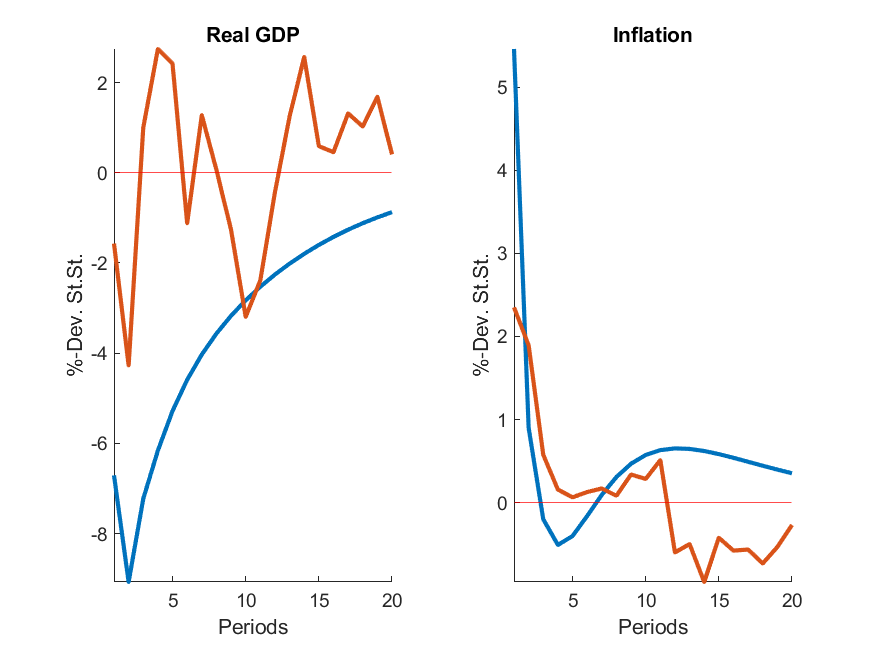
\includegraphics[width=0.7\textwidth]{../matlab_base/output/irf_gdp_taylor.png}
\end{figure}

\textbf{I THINK THAT THIS IS ALSO WHERE WE ADD OUR IMPULSE RESPONSE FUNCTIONS AS DESCRIBED IN THE INSTRUCTIONS!!!!}

% describe the short run as well as the path back to the steady state. 
\subsection*{(b) What is the idea behind the implemented policy (current policy scenario)?}

At the same time, in an effort to smooth out the path of the economy, the central bank will adjust the money supply to increase the purchasing power of the households and counter the shocks. By following the Taylor-like monetary policy rule, it will increase the money supply in order to match the inflation and marginal cost gaps of the economy in an effort to achieve price stability. As the bank intervention will increase the money stock of the households, it will allow it to consume more goods and therefore counter the drop in output that the economy experiences.\ \textbf{Think carefully about this, what is the ideal policy rule and how to actually best achieve price stability, what should the central bank target?}

\newpage
% 5. Counterfactual Policies
\section*{5. Counterfactual Policies (about two pages)}
\subsection*{(a) More or less of the same policy (different coefficients)?}
% Content here.

\subsection*{(b) Alternative policy (different targets)?}
% Content here.

% -------------------------------------------------------
%                       NOTES
% -------------------------------------------------------
% - try adding in the labour supply target instead of MC
% - think about implementing alternative inflation target (0.03)
% - think about alternative monetary policy rules 
% -  fiscal instead of monetary as a counter-factual?




% -------------------------------------------------------


% 6. Policy Recommendation and Discussion
\section*{6. Policy Recommendation and Discussion (about one page)}
\subsection*{(a) Give a recommendation on policy based on your simulations.}
% Content here.

\subsection*{(b) Should policy have taken a different path?}
% Content here.

\subsection*{(c) Do your results confirm or conflict with your perception about optimal policy? Discuss how.}
% Content here.
\printbibliography % Print the bibliography

% Appendix 
\appendix
\section*{Appendix A: Further Tables}
\begin{table}[ht]
    \centering
    \caption{Parameter Calibration}
    \begin{tabular}{clcl}
        \toprule
        Parameter & Description & Value & Source \\ \midrule
        %\hline \hline
        $\beta$ & Period discount factor  & 0.96 & - \\
        $\sigma$ & Intertemporal consumption elasticity  & $<1$ & - \\
        $\gamma$ & Inverse Frisch elasticity  & 3 & - \\
        $\nu$ & Money velocity  & 7 & - \\
        $\delta$ & Capital depreciation rate  & 0.1 & - \\
        $\phi_X$ & Investment adjustment cost parameter & - & - \\
        $\alpha$ & Capital share of income & 0.31 & - \\
        $\rho$ & Elasticity of substitution for differentiated goods &  0.38 & - \\
        $\kappa$ & Price stickiness & - & - \\
        $lg^Y_{ss}$ & Public-debt-to-GDP steady-state target & - & - \\
        ${\tau_L}$ & Labor income tax & - & - \\
        ${\tau_K}$ & Capital income tax & - & - \\
        ${\tau_C}$ & Consumption tax & - & -  \\
        ${\gamma_{l_g}}$ & Fiscal rule coefficient w.r.t. government liabilities & - & -  \\
        ${\theta_{\pi}}$ & Taylor coefficient w.r.t. inflation gap & 2 & - \\
        $\theta_R$ & Taylor coefficient w.r.t. interest rate & NA  & - \\  \bottomrule
    \end{tabular}
    \label{tab:parameters}
\end{table}

\end{document}